\documentclass{article}


\usepackage{conference}

\usepackage[utf8]{inputenc} % allow utf-8 input
\usepackage[T1]{fontenc}    % use 8-bit T1 fonts
\usepackage{hyperref}       % hyperlinks
\usepackage{url}            % simple URL typesetting
\usepackage{booktabs}       % professional-quality tables
\usepackage{amsfonts}       % blackboard math symbols
\usepackage{nicefrac}       % compact symbols for 1/2, etc.
\usepackage{microtype}      % microtypography
\usepackage[final]{graphicx}% graphics
\usepackage{lipsum}

\title{HOLOEXPO \emph{conference} preprint}
%{F.M. Sanchez,\ M. Grosmann,\ B. Kress,\ N. Flawisky,\ L. Gueroult, \textit{Cosmic Holography}}
\author{
  F.M. Sanchez~hol137\thanks{Use footnote for providing further
    information about author (webpage, alternative
    address)---\emph{not} for acknowledging funding agencies.} \\
  Department of Physics\\
  Paris 11 University\\
  Paris, FRANCE \\
  \texttt{hol137@yahoo.fr} \\
  %% examples of more authors
   \And
 M.H. Grosmann \\
  Department of Photonics\\
  University of Strasbourg\\
  Strasbourg, FRANCE \\
  \texttt{michel.grosmann@me.com} \\
  %% \AND
  %% Coauthor \\
  %% Affiliation \\
  %% Address \\
  %% \texttt{email} \\
  %% \And
  %% Coauthor \\
  %% Affiliation \\
  %% Address \\
  %% \texttt{email} \\
  %% \And
  %% Coauthor \\
  %% Affiliation \\
  %% Address \\
  %% \texttt{email} \\
}


\begin{document}
\maketitle

\begin{abstract}
\lipsum[1]
\end{abstract}


% keywords can be removed
\keywords{Quantum \and Holography \and Cosmos}


\section{Introduction}
\lipsum[2]
\lipsum[3]


\section{Section 1: first level}
\label{sec:headings}

\lipsum[4] See Section \ref{sec:headings}.

\subsection{Headings: second level}
\lipsum[5]
%\begin{equation}
%\xi _{ij}(t)=P(x_{t}=i,x_{t+1}=j|y,v,w;\theta)= {\frac {\alpha _{i}(t)a^{w_t}_{ij}\beta _{j}(t+1)b^{v_{t+1}}_{j}(y_{t+1})}%{\sum _{i=1}^{N} \sum _{j=1}^{N} \alpha _{i}(t)a^{w_t}_{ij}\beta _{j}(t+1)b^{v_{t+1}}_{j}(y_{t+1})}}
%\end{equation}

\subsubsection{Headings: third level}
\lipsum[6]

\paragraph{Paragraph}
\lipsum[7]

\section{Examples of citations, figures, tables, references}
\label{sec:others}
\lipsum[8] \cite{Sanchez3,Sanchez4} and see \cite{Grosmann}.

The documentation for \verb+natbib+ may be found at
\begin{center}
  \url{http://mirrors.ctan.org/macros/latex/contrib/natbib/natnotes.pdf}
\end{center}
Of note is the command \verb+\citet+, which produces citations
appropriate for use in inline text.  For example,
\begin{verbatim}
   \citet{hasselmo} investigated\dots
\end{verbatim}
produces
\begin{quote}
  Hasselmo, et al.\ (1995) investigated\dots
\end{quote}

\begin{center}
  \url{https://www.ctan.org/pkg/booktabs}
\end{center}


\subsection{Figures}
\lipsum[10] 
See Figure \ref{fig:figure_label}. For more explanations. \footnote{Sample of the first footnote.}
\lipsum[11] 

\begin{figure}
  \centering
  %\fbox{\rule[-.5cm]{4cm}{4cm} \rule[-.5cm]{4cm}{0cm}}
  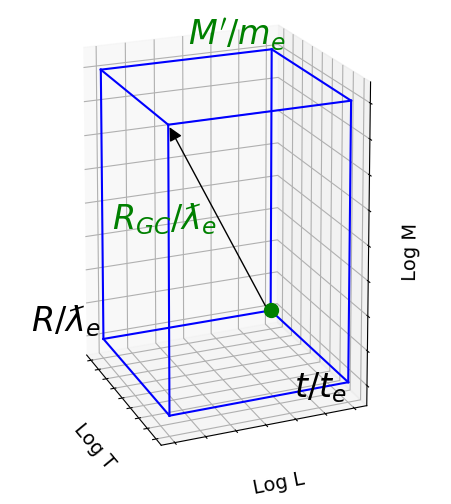
\includegraphics[width=15cm,height=16cm]{./figures/triaxis.png}
  \caption{Geo dimensional Universe-Grandcosmos couple. In a 3D Super-space, natural logarithms of length, time and mass ratios are considered as vectors. The logarithm of ratio of Grandcosmos radius by the Compton electron wavelength appears as the norm of the vector using for length and time projections a common ratio, that of the Hubble radius by the electron Compton wavelength, and for mass ratio that of $M^{\prime}$ by the electron mass. $M^{\prime}$ being the critical mass in the Grandcosmos reduced spherical hologram, this is a dramatic geometrical confirmation of the Extended (2D-1D) Holographic Principle applied to the Bekenstein-Hawking Universe entropy. The Grandcosmos existence cannot be denied since the relation between $e$, $a$ and involved logarithms reach precision $10^{-7}$.}
  \label{fig:figure_label}
\end{figure}

\subsection{Tables}
\lipsum[12]
See awesome Table~\ref{tab:table}.

\begin{table}
 \caption{Sample table title}
  \centering
  \begin{tabular}{lll}
    \toprule
    \multicolumn{2}{c}{Part}                   \\
    \cmidrule(r){1-2}
    Name     & Description     & Size ($\mu$m) \\
    \midrule
    Dendrite & Input terminal  & $\sim$100     \\
    Axon     & Output terminal & $\sim$10      \\
    Soma     & Cell body       & up to $10^6$  \\
    \bottomrule
  \end{tabular}
  \label{tab:table}
\end{table}

\subsection{Lists}
\begin{itemize}
\item Lorem ipsum dolor sit amet
\item consectetur adipiscing elit. 
\item Aliquam dignissim blandit est, in dictum tortor gravida eget. In ac rutrum magna.
\end{itemize}

\begin{figure}
  \centering
  %\fbox{\rule[-.5cm]{4cm}{4cm} \rule[-.5cm]{4cm}{0cm}}
  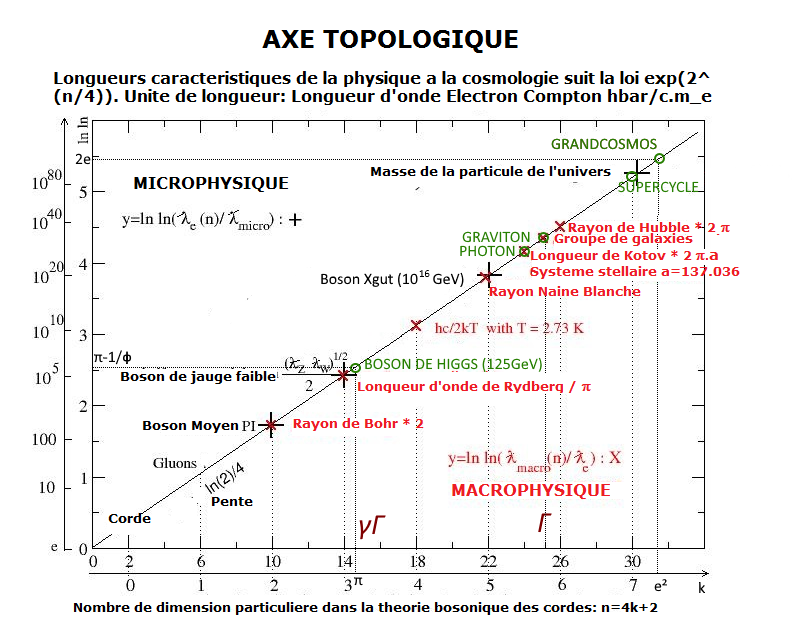
\includegraphics[width=15cm,height=16cm]{./figures/figure.png}
  \caption{The Topological Axis. Double natural logarithms (y = lnln(Y)) of main dimensionless physical quantities 
(Y) corresponds to the String dimension series n = 4k + 2, from k = 0 to k = 7, showing the Bott
periodicity 8 [19] which is at the origin of the name `Topological Axis.}
  \label{fig:figure_label}
\end{figure}

\bibliographystyle{unsrt}  
%\bibliography{references}  %%% Remove comment to use the external .bib file (using bibtex).
%%% and comment out the ``thebibliography'' section.


%%% Comment out this section when you \bibliography{references} is enabled.
\begin{thebibliography}{1}

\bibitem{Sanchez3} Sanchez F.M. ``Towards the grand unified Holic Theory''. Current
Issues in Cosmology. Ed. J.-C. Pecker and J. Narlikar. Cambridge Univ. Press,
2006; p. 257--260.

\bibitem{Sanchez4} Sanchez F; M. ``Holic Principle: The coherence of the Universe`` (Sept 1995), Entelechies, 16th ANPA, 324--344.

\bibitem{Grosmann} Grosmann, M. and Meyrueis P. ``Optics and Photonics Applied to Communication and Processing''. SPIE.  Jan 1979.
\newblock Optics and Photonics Applied to Communication and Processing.
\newblock In {\em SPIE (SPIE), 1979 
  International Conference on}, pages . SPIE, 1979.

\bibitem{Grosmann2} Grosmann, M and Rebordão, José and Meyrueis, Patrick, 1985,02,p761--765,Propagation Of Waves In Optical Systems: Reformulation Of Huyghens Principle For Aspheric Systems,
volume 491, Proceedings of SPIE - The International Society for Optical Engineering, doi:10.1117/12.968010

\bibitem{Kress} Digital Diffractive Optics: An Introduction to Planar Diffractive Optics and Related Technology, by B. Kress, P. Meyrueis, pp. 396. ISBN 0-471-98447-7. Wiley-VCH , October 2000.
\newblock An Introduction to Planar Diffractive Optics and Related Technology.

\bibitem{Sanchez5} F.M. Sanchez, V. Kotov, M. Grosmann, D. Weigel, R. Veysseyre, C. Bizouard, N. Flawisky, D. Gayral, L. Gueroult, Back to Cosmos
\newblock {\em arXiv preprint viXra:1904.0218}, 2019.

\end{thebibliography}


\end{document}
